%% LaTex
%%
%%
%% Title: C-SAFE homebrew documentation
%%
%% Authors: Steve Parker, others later
%%
%%%%%%%%%%%%%%%%%%%%%%%%%%%%%%%%%%%%%%%%%%%%%%%%%%%%%%%%

\documentclass[11pt]{article}
%%\documentclass[widereview,draft]{/home/crj/papers/cls/IEEEtran}
\usepackage{times}              % Postscript fonts.
\usepackage{epsfig}
\usepackage{program}
%\usepackage{latexsym}
%\usepackage{amsmath}
\oddsidemargin 0in
\textwidth 6.5in
\topmargin -.5in
\textheight 9in


%%\documentstyle[11pt,draft,epsf,amstex]{ieeetran}
%%\documentstyle[11pt,epsf,draft,titlepage]{article}

%%%%%%%%%%%%%%%%%%%%%%%%%%%%%%%%%%%%%%%%%%%%%%%%%%%%%%%%%%%%%%%%%%%%
%%
%% Put text into a box centered on the page.
%%
%%       \boxtext{...}           
%%       \boxtextcenter{...}     % center text in box (short message!)
%%       \boxtexthighlight{...}  % center bold text in box (short message!)%
%%%%%%%%%%%%%%%%%%%%%%%%%%%%%%%%%%%%%%%%%%%%%%%%%%%%%%%%%%%%%%%%%%%%%
                                %
\newdimen\boxtextwidth
\setlength{\boxtextwidth}{\columnwidth}
\newcommand{\boxtext}[1]{\hfill\rule{0ex}{0.01ex}
  \centerline{\fbox{\parbox{\boxtextwidth}{#1}}}}
\newcommand{\boxtextcenter}[1]{\boxtext{\centerline{#1}}}
\newcommand{\boxtexthighlight}[1]{\boxtextcenter{\textbf{#1}}}
                                %
%%%%%%%%%%%%%%%%%%%%%%%%%%%%%%%%%%%%%%%%%%%%%%%%%%%%%%%%%%%%%%%%%%%%%

\begin{document}


\title{Towards Homebrew 1.0}


\author{ Steven G. Parker, others in the future
      }

\maketitle


\tableofcontents

\begin{abstract}




\end{abstract}

\newpage

%%
%% INTRODUCTION
%%

% -*-latex-*-
%
%  The contents of this file are subject to the University of Utah Public
%  License (the "License"); you may not use this file except in compliance
%  with the License.
%
%  Software distributed under the License is distributed on an "AS IS"
%  basis, WITHOUT WARRANTY OF ANY KIND, either express or implied. See the
%  License for the specific language governing rights and limitations under
%  the License.
%
%  The Original Source Code is SCIRun, released March 12, 2001.
%
%  The Original Source Code was developed by the University of Utah.
%  Portions created by UNIVERSITY are Copyright (C) 2001, 1994
%  University of Utah. All Rights Reserved.
%

% intro.tex
%

\chapter{Introduction}
\label{ch:intro}


This is the \etitle{\srug}.  It describes the purpose and use of the
\sr{} problem solving environment (\pse).  This guide is for users who
are building and executing \dfn{networks} within the \sr{}
environment.

Users installing \sr{} should read the
\htmladdnormallinkfoot{\srig}{\htmlurl{\latexhtml{\scisoftware/doc}{../../..}/Installation/Guide/ch.inst.html}}.

Users of the BioTensor Power App should see the
\htmladdnormallinkfoot{BioTensor
  tutorial}{\latexhtml{http://software.sci.utah.edu/doc/User/Tutorials/BioTensor/BioTensor.html}{../../Tutorials/BioTensor/BioTensor.html}}.

%\section{Conventions}
%\label{sec:conventions}

%\missing{Discussion of typographic conventions}

\section{Road Map}
\label{sec:roadmap}

This document is organized into the following sections:

\begin{description}
  \descitem{\chref{Introduction}{ch:intro}} This introduction.
  
  \descitem{\chref{Concepts}{ch:concepts}} Introduces the concept of
  an integrated problem solving environment and describes how \SR{}
  embodies these ideas.
  
  \descitem{\chref{Packages}{ch:packages}} Gives an overview
  of the \sr{} and \biopse{} packages.
  
  \descitem{\chref{Starting \sr}{ch:startingup}} Outlines procedure
  for starting \sr{} and related information.

  \descitem{\chref{Working with Networks}{ch:workwithnets}}
  Discusses building, editing, and executing
  networks.

  \descitem{\chref{Visualization}{ch:viewer}}
  Describes the purpose and use of the \viewer{} (visualization) module.

  \descitem{\chref{Importing data into \sr{}}{ch:import_export}}
  Describes ways to import/export ``foreign'' data into/out of \SR{}.
\end{description}

\section{Help}
\label{sec:help}

Help is available from the following sources.

\subsection{Documentation Distribution}

\sr{} documentation is distributed separately from its source code.
\sr{}'s documentation distribution can be downloaded from
\htmladdnormallinkfoot{\sr{}'s software download
  page}{\scisoftwarearchiveurl}.  See the 
\htmladdnormallinkfoot{\srig}{\htmlurl{\latexhtml{\scisoftware/doc}{../../..}/Installation/Guide/ch.inst.html}}
for instructions on downloading and installing the documentation
distribution.

After installing the documentation, point the browser at the
\filename{index.html} file located in the distribution's top level
\directory{doc} directory (\ie{} \ab{top of documentation
  distribution}/doc/index.html).

\subsection{The Web}

This and other documents related to \sr{} can be found 
\htmladdnormallinkfoot{online}{\scidocurl{}}.

Visit the \sci{} web site for more
information related to \sr{} and the \scii{}.

\subsection{Mailing Lists}

The \sr{} \emph{users} mail list is a forum for discussing \sr{}
related issues.  To subscribe send mail to:

\mailto{Majordomo@sci.utah.edu}

with the following command in the body of the message:

\keyboard{subscribe scirun-users}

After subscribing,  questions can be sent to
\mailto{scirun-users@sci.utah.edu}.

The \sr{} \emph{developers} list is a forum for network and module
developers.  To subscribe send mail to:

\mailto{Majordomo@sci.utah.edu}

with the following command in the body of the message:

\keyboard{subscribe scirun-develop}

After subscribing, questions can be sent to
\mailto{scirun-develop@sci.utah.edu}.

\section{Reporting Bugs}
\label{sec:bugs}

Please report bugs!  To report a bug visit \sr{}'s
\htmladdnormallinkfoot{bug database}{\bugsurl} web page.

Reporting bugs to the bug database, rather than the mailing list,  ensures
bugs are fixed in a timely manner.

%%% Local Variables: 
%%% mode: latex
%%% TeX-master: "usersguide"
%%% End: 


\section{Uintah-specific Libraries}

\documentclass[12pt]{article}
\usepackage[dvips]{graphicx}

%%%%% My macros - get rid of them later if needed.

\newcommand{\single }{\renewcommand{\baselinestretch}{1} \large \normalsize}
\newcommand{\hdouble}{\renewcommand{\baselinestretch}{1.5} \large \normalsize}
\newcommand{\double }{\renewcommand{\baselinestretch}{1.66} \large \normalsize}

\begin{document}

%\double

\begin{figure}[htbp]
%\begin{center}
\hskip -3.4cm
\includegraphics[width=1.5\textwidth]{grid.eps}
%\end{center}
\caption{AMR Grid Layout.}
\label{grid}
\end{figure}  

\end{document}


\section{Support for Parallelism}


\section{Components}



\end{document}
